\documentclass[a4paper, 11pt]{article}
\usepackage[utf8]{inputenc}
\usepackage{graphicx}
%\usepackage{amsfont}
\usepackage{amsmath}
\usepackage{amssymb}
\usepackage{hyperref}
%\usepackage[french]{babel}

\begin{document}

\title{Moteur de lancer de rayons}
\author{Coiffier Guillaume - Béthune Louis - Felderhoff Joël}
\date{Janvier 2017} 

\maketitle

\section*{Présentation (cf Wikipedia)}
 
Le \textit{Raytracing} (ou lancer de rayons en québecois supérieur) est une méthode de rendu de scènes 3D. Il permet d'obtenir des images d'excellente qualité en simulant le comportement naturel de la lumière : réflexions, ombres, changement d'indice, diffusion, éclairage, flou de profondeur... 
  
La théorie sur le domaine est assez ancienne (années 60) mais l'exigence de cette méthode en terme de charge de calcul ont longtemps limité son usage. Cette technologie a donc connu une renaissance dans les années 2000, notamment dans le cinéma d'animation ou la simulation scientifique.  
  
C'est une technique assez simple à mettre en œuvre et on obtient rapidement des résultats, même si un moteur complet (comme celui ayant produit l'image ci-dessous) nécessite un travail titanesque.

\begin{center}
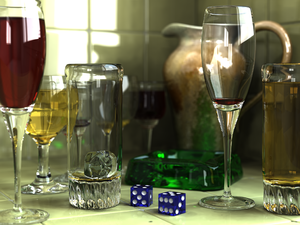
\includegraphics[scale=1]{300px-Glasses_800_edit.png}
\end{center}
\newpage

\section{Principe}
L'idée est de simuler le comportement d'un rayon lumineux, en utilisant le principe du parcours inverse de la lumière.  
  
Ainsi, pour chaque pixel de la caméra, on lance un rayon et on cherche le premier objet qu'il intersecte. On peut alors afficher ce pixel de la couleur de l'objet. 
  
\begin{center}
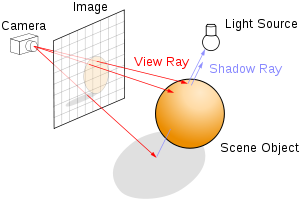
\includegraphics[scale=0.8]{300px-Ray_trace_diagram.png} 
\end{center}

On peut prendre en compte l'éclairage de façon très simple : on calcule les coordonnées du point d'intersection, puis on "tire" un rayon imaginaire en direction de la source de lumière. Si ce rayon atteint la source de lumière, le pixel apparaît éclairé. Dans le cas contraire, si on intersecte un autre objet de la scène, alors il y a occlusion et le pixel apparaît en sombre.  

\begin{center}
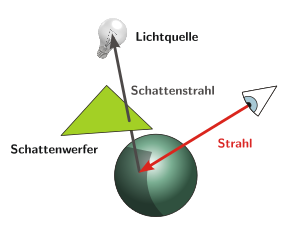
\includegraphics[scale=0.8]{290px-Raytracing-Schattenstrahl.png} 
\end{center}
\newpage

\section{Votre mission}
\subsection*{Niveau 1 : le z-buffer}

Implémentez un raytracer élémentaire. Pour cela vous devez supporter :  
  
\begin{description}
\item [Une caméra] simple unidirectionnelle, de normale orientée selon l'axe z et centrée en $(0, 0, 0)$
\item [Des objets simples] comme des sphères monochromatique. Pensez à une architecture assez souple pour pouvoir gérer d'autres formes plus tard. 

Équation décrivant un rayon : $ t\in \mathbb{R}, d\in \mathbb{R}^3, O + dt$ où $d$ est la direction
 
Équation décrivant une sphère : $(x - x_0)^2 + (y - y_0)^2 + (z - z_0)^2 = R^2$ de centre $(x_0, y_0, z_0)$ et de rayon $R$
\item [Un z-buffer] pour prendre en compte la profondeur. Les objets proches doivent être affichés avec des couleurs vives, et les objets lointains avec des couleurs sombres. 
  
\end{description}  

\subsection*{Niveau 2 : d'autres formes et des couleurs}

Rajoutez :

\begin{description}
\item [D'autres formes] comme des triangles par exemple. Intéressez vous à l'algorithme de \textit{Moller Trumbore}.  
\item [De la couleur] sur vos objets. Prévoyez une architecture assez souple pour gérer des matériaux plus compliqués plus tard (surfaces réfléchissantes, textures).  
  
\end{description}  

\textbf{Exemple :}
  
\begin{center}
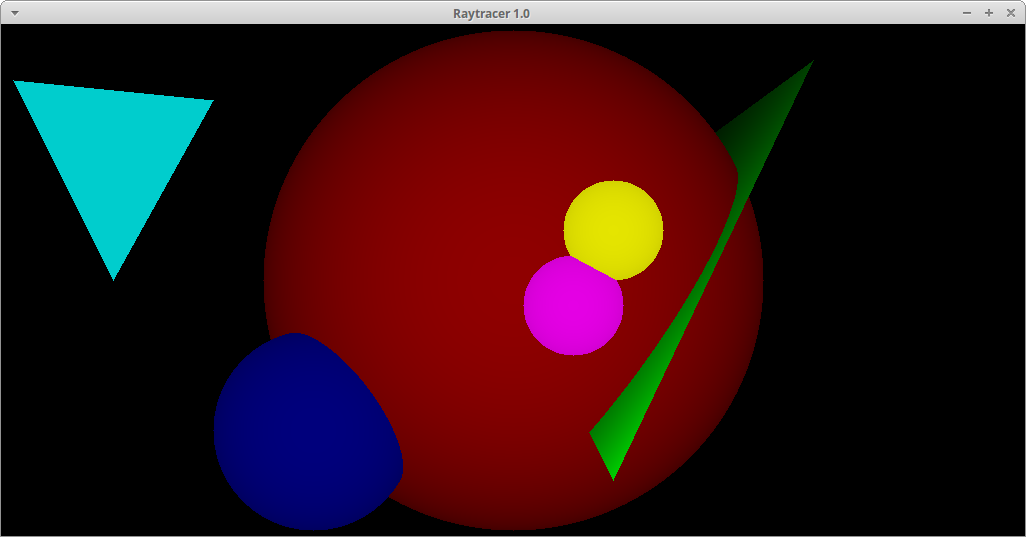
\includegraphics[scale=0.2]{correct1.png} 
\end{center}

\section*{Conseils}  
\subsection{Architecture}  
  
Pensez que votre moteur va évoluer. L'idée est de mettre en pratique tout ce que vous avez appris en terme de programmation orientée objet et de généricité pour créer quelque chose adaptatif et évolutif. Pensez par exemple à une interface IForme pour vos différentes formes, et posez vous les questions suivantes : qu'est ce qui caractérise mon objet ? quel est son essence ? Si vous codez en vous posant ces questions, votre architechture ne peut que tendre vers le bon.

\subsection{Travail à plusieurs}
Autre chose : une solution pour travailler vite et avoir quelque chose de plus puissant est de travailler à plusieurs. Parlez en à votre TDman/TDgirl et profitez en pour apprendre à travailler à plusieurs sur un même code : regardez du coté de Git.

\subsection{Bibliothèque et langage}  
  
La bibliothèque standard du C++ ne propose pas nativement de moyens de faire du fenêtrage ou des applications graphiques. Il vous faudra donc une bibliothèque extérieure, dont il faudra apprendre la documentation et le fonctionnement.

Il en existe des dizaines mais je suggère à titre personnel la SFML(\url{https://www.sfml-dev.org/index-fr.php}) qui est :  
  
\begin{itemize}
\item simple à utiliser et très intuitive, peu volumineuse
\item suffisamment rapide pour l'usage que l'on va en faire
\item entièrement orientée objet
\item exploitant les mécanismes du C++ idiomatique comme la RAII
\item développée par un français, avec des tutoriels en français et une communauté francophone active
\item multi-plateforme
\end{itemize}

\end{document}
